\usepackage{hyperref}

%!TEX root = ../Thesis.tex
\section{Projekt-Architektur}\label{Projekt-Architektur}
Die Ordnerstruktur des Projekts ist in \autoref{fig:dir_struc_root} zu sehen. Die Strukturen für das Frontend, Backend
sowie den NodeMCU Code sind in \autoref{anh:Projekt-Architektur} zu finden.
\begin{figure}[H]
    \centering
    \begin{minipage}[t]{1\textwidth}
        \caption{Root-Ordnerstruktur}
        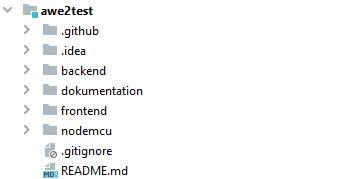
\includegraphics[width=0.5\textwidth]{img/dir_struc_root.png}\\
        \source{Eigene Darstellung}
        \label{fig:dir_struc_root}
    \end{minipage}
\end{figure}





